

\begin{frame}
\frametitle{Private registry}
A local Docker registry can be useful in many situations
\begin{itemize}
\item images contain private data or information
\item need to test specific applications
\item speed and reliability
\item other applications require the service
\end{itemize}
\end{frame}


\begin{frame}
\frametitle{Private registry}
A local Docker registry can be useful in many situations
\begin{itemize}
\item images contain private data or information
  \begin{itemize}
  \item passwords
  \item user names
  \item network configurations
  \item mount points
  \end{itemize}
\item need to test specific applications
\item speed and reliability
\item other applications require the service
\end{itemize}
\end{frame}


\begin{frame}
\frametitle{Private registry}

A local Docker registry can be useful in many situations

\begin{itemize}
\item images contain private data or information
\item need to test specific applications
\item speed and reliability
  \begin{itemize}
  \item good internet connection
  \item not limited by number of images or containers
  \item lots of disk space
  \end{itemize}
\item other applications require the service
\end{itemize}
\end{frame}


\begin{frame}
\frametitle{Private registry}

A local Docker registry can be useful in many situations

\begin{itemize}
\item images contain private data or information
\item need to test specific applications
\item speed and reliability
\item other applications require the service
  \begin{itemize}
  \item workflow managers may use Docker container for running the pipelines
  \item other container technologies depends on custom Docker images
  \end{itemize}
\end{itemize}
\end{frame}


\begin{frame}[fragile]
\frametitle{Docker Registry}
\framesubtitle{run}
Run an insecure registry

\begin{lstlisting}
$ docker run -d -p 5000:5000 \
           --restart=always \
		   --name registry registry:2
\end{lstlisting}

\textit{!!! WARNING !!!} this is an insecure registry.
\end{frame}

\begin{frame}[fragile]
\frametitle{Docker Registry}
\framesubtitle{run}
Run an insecure registry

\begin{lstlisting}
$ docker run -d -p 5000:5000 \
           --restart=always \
		   --name registry registry:2
\end{lstlisting}

This registry runs on the localhost

and
\end{frame}

\begin{frame}[fragile]
\frametitle{Docker Registry}
\framesubtitle{run}
Run an insecure registry

\begin{lstlisting}
$ docker run -d -p 5000:5000 \
           --restart=always \
		   --name registry registry:2
\end{lstlisting}
This registry runs on the localhost

and

is \textit{INSECURE} but it's OK for testing.
\end{frame}

\begin{frame}[fragile]
\frametitle{Docker Registry}
\framesubtitle{run}

Check if the registry is running

\begin{lstlisting}
$docker ps
CONTAINER ID  IMAGE      COMMAND
d37dd351dd30  registry:2 "/entrypoint.sh /e..."

CREATED    STATUS    PORTS                  
15 min ago Up 15 min 0.0.0.0:5000->5000/tcp 

NAMES
registry
\end{lstlisting}
\end{frame}

\begin{frame}[fragile]
\frametitle{Docker Registry}
\framesubtitle{load an image}

Get an image from the net

\begin{lstlisting}
$ docker pull ubuntu:18.04
\end{lstlisting}
\end{frame}

\begin{frame}[fragile]
\frametitle{Docker Registry}
\framesubtitle{load an image}

Tag the image with a proper name
\begin{lstlisting}
$ docker tag ubuntu:18.04 \
    localhost:5000/user/mydistro:18.04
    
\end{lstlisting}
\end{frame}

\begin{frame}[fragile]
\frametitle{Docker Registry}
\framesubtitle{load an image}

Push the image to the local repository

\begin{lstlisting}
$ docker push \
  localhost:5000/user/mydistro:18.04
\end{lstlisting}
\end{frame}

\begin{frame}[fragile]
\frametitle{Docker Registry}
\framesubtitle{list images}

Docker works with HTTP API (v2)

\begin{lstlisting}
$ curl -v http://localhost:5000/v2/_catalog
\end{lstlisting}

\url{https://docs.docker.com/registry/spec/api/}

\end{frame}

\begin{frame}[fragile]
\frametitle{Docker Registry}
\framesubtitle{list images}

\begin{lstlisting}
< HTTP/1.1 200 OK
< Content-Type: application/json; charset=utf-8
< Docker-Distribution-Api-Version: registry/2.0
< X-Content-Type-Options: nosniff
< Date: Tue, 25 Sep 2018 13:36:04 GMT
< Content-Length: 52
<
{"repositories":["joe/ubuntu","raoul/ubuntu"]}
* Connection #0 to host localhost left intact
\end{lstlisting}
\end{frame}

\begin{frame}[fragile]
\frametitle{Docker Registry}
\framesubtitle{get tags}

\begin{lstlisting}
$ curl http://localhost:5000/raoul/ubuntu/tags/list
{"name":"raoul/ubuntu","tags":["18.04"]}
\end{lstlisting}
\end{frame}

\begin{frame}[fragile]
\frametitle{Docker Registry}
\framesubtitle{get details}

\begin{lstlisting}
$ curl http://localhost:5000/raoul/ubuntu/manifests/18.04
\end{lstlisting}

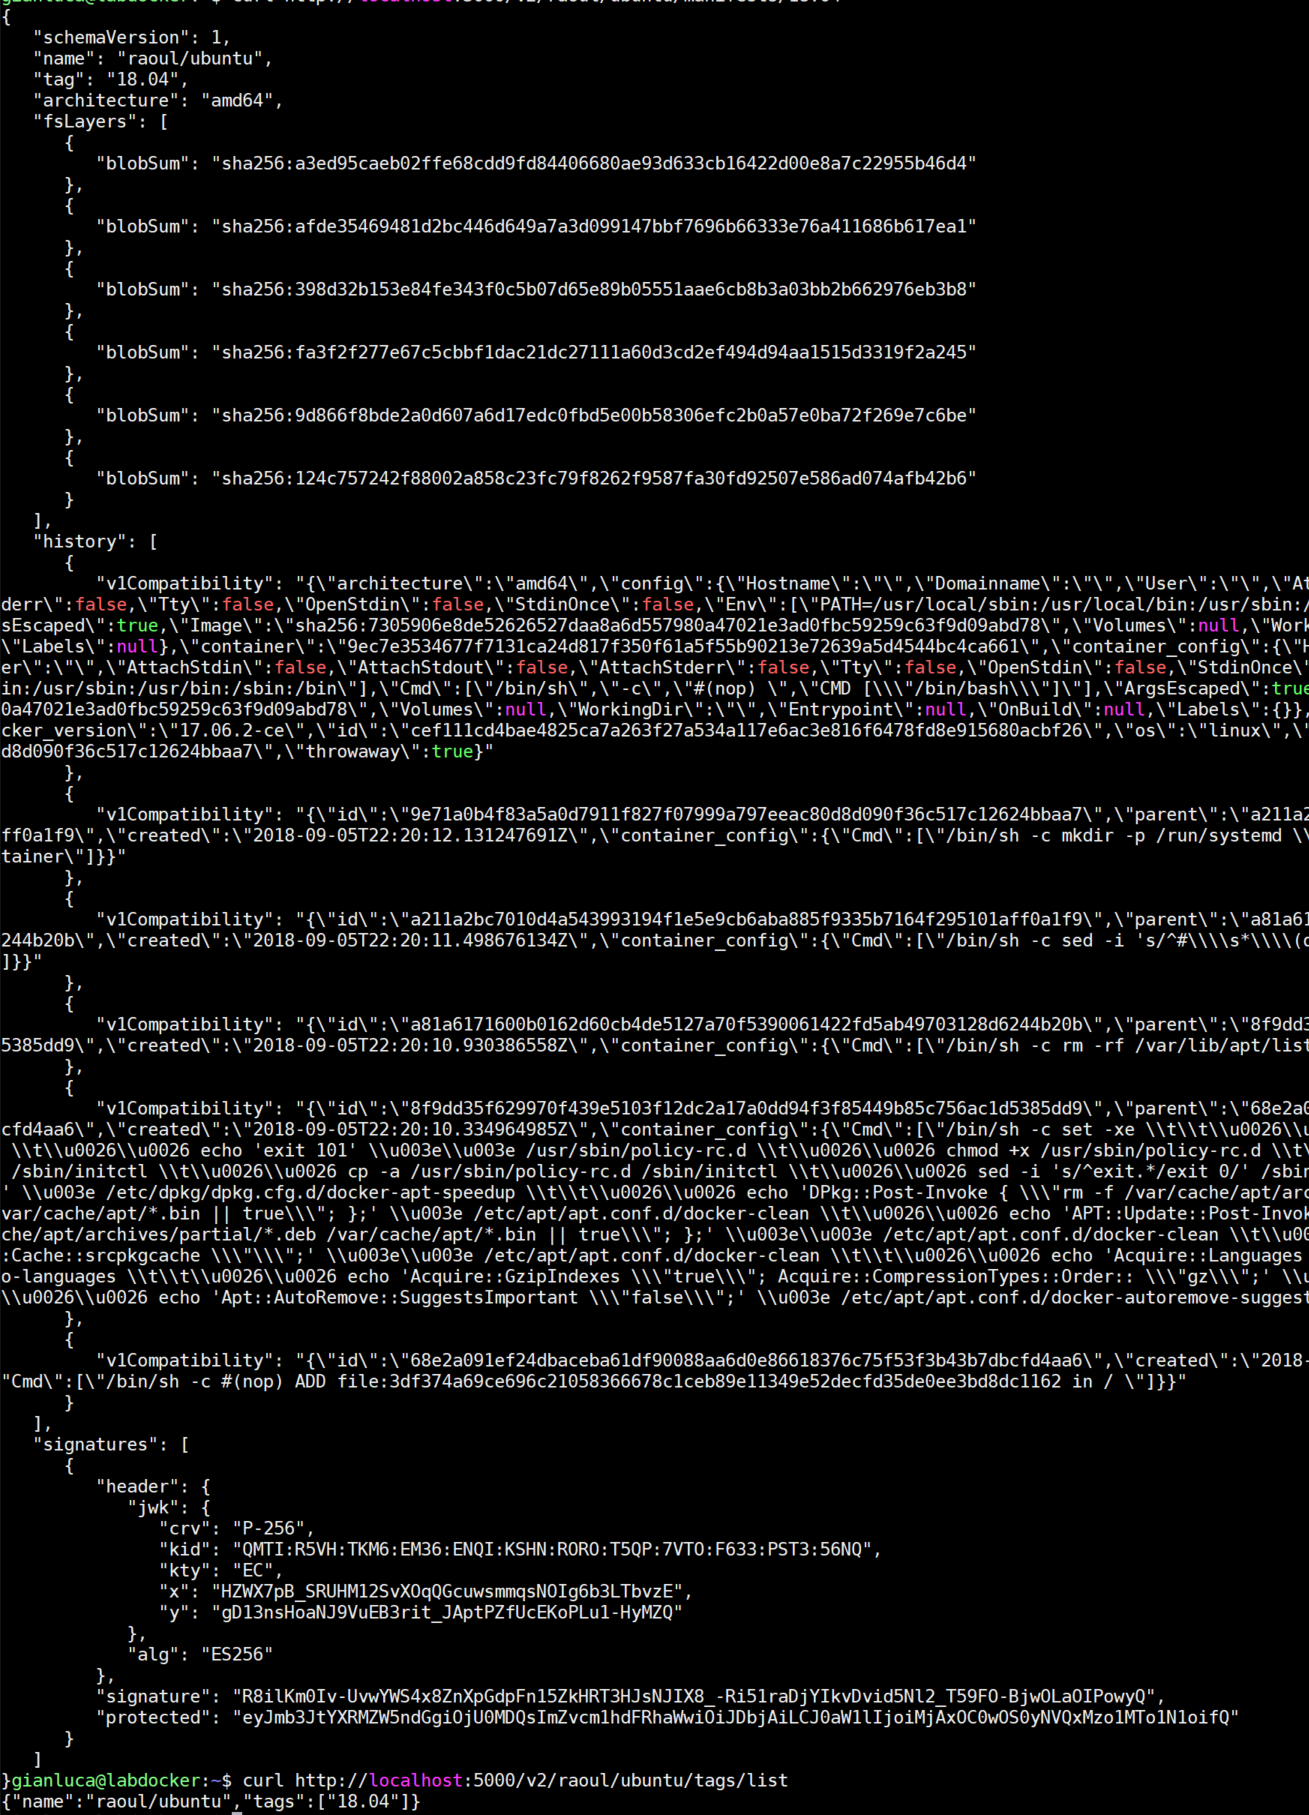
\includegraphics[width=0.8\columnwidth]{./Figure/RegistryDetails}
\end{frame}

\begin{frame}[fragile]
\frametitle{Docker Hub}
\framesubtitle{public registry}

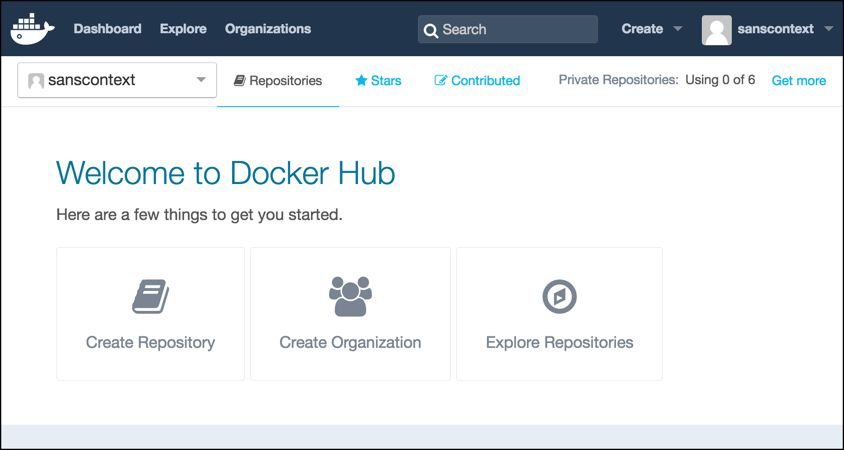
\includegraphics[width=0.8\columnwidth]{./Figure/docker-222-114}
\end{frame}


\begin{frame}[fragile]
\frametitle{Docker Hub}
\framesubtitle{public registry}

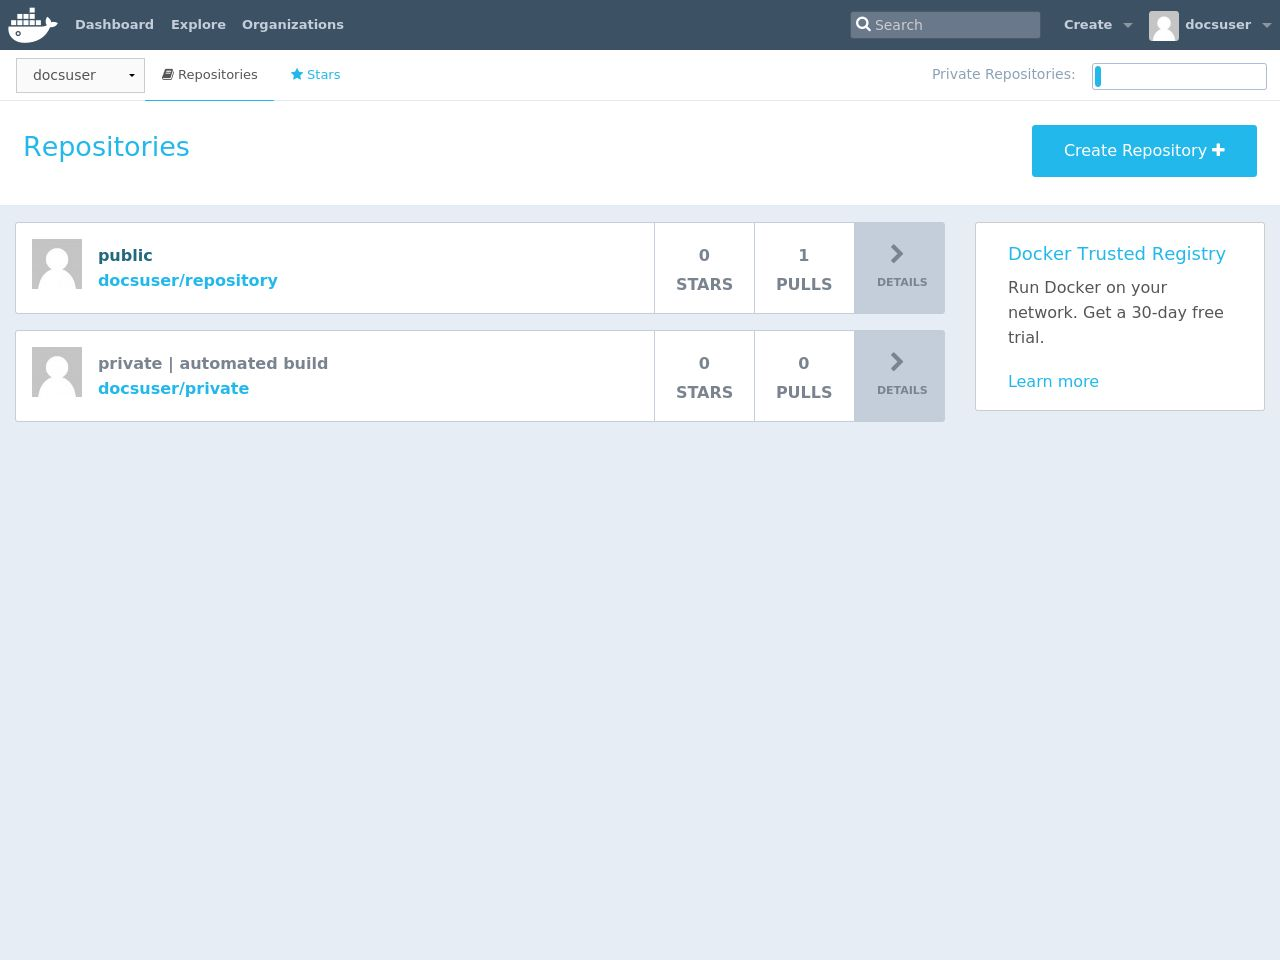
\includegraphics[width=0.8\columnwidth]{./Figure/docker-223-116}
\end{frame}

\begin{frame}[fragile]
\frametitle{Docker Hub}
\framesubtitle{public registry}
\begin{itemize}
\item register a new user to \url{https://hub.docker.com/}
\item \lstinline!export DOCKER_ID_USER="username"!
\item \lstinline!docker login!
\item \lstinline!docker tag imageX $DOCKER_ID_USER/imageX!
\item \lstinline!docker push $DOCKER_ID_USER/imageX!
\end{itemize}
\end{frame}